\begin{frame}{Detecting plants on soil background.}

Defining a measure based on normalized RGB intensities:
\begin{columns}
\begin{column}{0.3\textwidth}

{\tiny
$$ExG=2{\color{green}G}-{\color{red}R}-{\color{blue}B}$$
$$CIVE = 0.441{\color{red}R} - 0.811{\color{green}G} + 0.385{\color{blue}B} + 18.787$$
$$MExG=1.262{\color{green}G}-0.884{\color{red}R}-0.311{\color{blue}B}$$}
\includegraphics[width=\linewidth]{pics/seg}
\end{column}
\begin{column}{0.69\textwidth}
\begin{center}
\includegraphics[width=\linewidth]{pics/cidx}
\end{center}
\end{column}
\end{columns}

Distributions with 2 well separated peaks: successful semgentation into background and plants (after filtering out the small patches)

{\tiny [Hamuda et al. A Survey of Image Processing Techniques for Plant Extraction and Segmentation in the Field. Comput. Electron. Agric., 2016]}

\end{frame}

\begin{frame}{Robustness of the segmentation segmentation.}

\begin{columns}
\begin{column}{0.45\textwidth}
\cutpic{2.5cm}{.8\linewidth}{pics/tpath}
\end{column}
\begin{column}{0.5\textwidth}
Usually sufficient to drive the weeding tool. 
\end{column}
\end{columns}

\begin{itemize}
\item Maybe limited for fine analysis of plant shapes.
\item Not robust to various light conditions or contexts.
\end{itemize}

\includegraphics[width=.65\linewidth]{pics/mask_pb}
\includegraphics[width=.3\linewidth]{pics/trihist2}

=> use of annotated data

\end{frame}

\begin{frame}{Learning methods for segmentation.}

\begin{itemize}
\item Learned classifiers (Random forest, support vector machine) based on context, 
\item Convolutional neural network (SegNet). 
\end{itemize}

\includegraphics[width=\linewidth]{pics/segnet}

Dataset?

\hfill {\tiny  Vijay Badrinarayanan, Alex Kendall and Roberto Cipolla SegNet: A Deep Convolutional Encoder-Decoder Architecture for Image Segmentation. PAMI, 2017}
\end{frame}

\begin{frame}{Shortcuts for building datasets.}

\begin{columns}
\begin{column}{0.3\textwidth}
\begin{itemize}
\item External annotated datasets.
\item<2-3> Transfer knowledge fom generic networks
\end{itemize}
\end{column}
\begin{column}{0.65\textwidth}
\only<1>{
\begin{columns}
\begin{column}{0.3\textwidth}
{\tiny CVPPP 2017 Challenge}\\
\includegraphics[width=\linewidth]{pics/rgb}\\
\includegraphics[width=\linewidth]{pics/fg}\\\includegraphics[width=\linewidth]{pics/label} 
\end{column}
\begin{column}{0.65\textwidth}
{\tiny [Giselsson et al. A Public Image Database for Benchmark of Plant Seedling Classification Algorithms, 2017]}\\
\hfill \includegraphics[width=.27\linewidth]{pics/rig}\\
\includegraphics[width=.48\linewidth]{pics/pdata_rgb}
\includegraphics[width=.48\linewidth]{pics/pdata_fg}\\
\end{column}
\end{columns}

}
\only<2>{
Common objects in context (COCO) datset
\includegraphics[width=\linewidth]{pics/coco-examples}
{\tiny Ren et al. Faster R-CNN: Towards Real-Time Object Detection with Region Proposal Networks, NIPS 2015}\\
\includegraphics[width=.48\linewidth]{pics/fastrcnn}
\includegraphics[width=.48\linewidth]{pics/frcnn_det}
}

\only<3>{
\begin{itemize}
\item Syntetic dataset
\item Building large datasets from few annotations (weakly supervised learning,...)
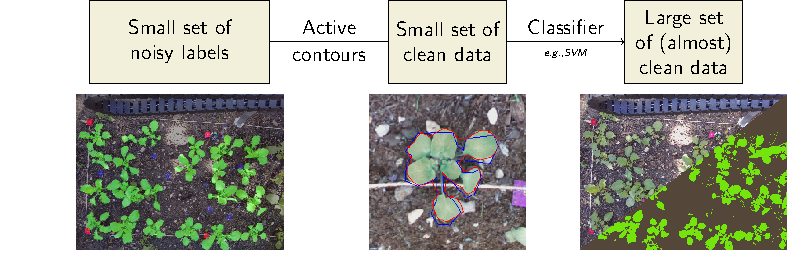
\includegraphics[width=\linewidth]{pics/data_curation}

\end{itemize}}
\end{column}
\end{columns}

\end{frame}
